\documentclass[11pt]{article}
\usepackage[utf8]{inputenc}
\usepackage{graphicx}
\graphicspath{ {images/} }
\usepackage{amsmath}
\usepackage{placeins}

\title{Coursework 1 – Transient Conduction}
\author{Adam Duncan}
\date{\today}

\begin{document}

\maketitle

\section{\emph{Part A: Using lumped capacitance}}
\subsection{Assumptions}
\begin{itemize}
	\item Internal temperature of the steel ball is uniform at any time t.
	\item No change in water temperature
	\item No heat transfer by radiation
	\item Material is standard carbon steel
	\item Material properties constant (taken at average temperature $T = 469 ^{o}C$)
\end{itemize}
\subsection{Properties}
\begin{table}[h]
	\centering
	\caption{Properties from problem}
	\begin{tabular}{lllll}
		Property & Value & Unit &  &  \\ \cline{1-3}
		Characteristic   length, L & 5 & cm &  &  \\
		Diameter, D & 10 & cm &  &  \\
		Temperature   of the water, $T_w$ & 38 & $^oC$ &  &  \\
		Initial   temperature of steel ball, $T_{s,1}$ & 900 & $^oC$ &  &  \\
		Final   temperature of steel ball, $T_{s,2}$ & 200 & $^oC$ &  &  \\
		Heat transfer   coefficient, h & 600 & $W/m^{2}K$ &  & 
	\end{tabular}
	\label{tab1}
\end{table}

\begin{table}[h]
	\centering
	\caption{Properties from literature}
	\begin{tabular}{llll}
		Property & Value at $T_{avg}$(469 $^{o}C$) & Unit & Source \\ \hline
		Specific heat   capacity, Cp & 552 & J/kgK &  \\
		Density & 7.8 x $10^3$ & $kg/m^3$ &  \\
		Conductivity & 40 & W/mK & 
	\end{tabular}
	\label{tab2}
\end{table}
\FloatBarrier

\subsection{Schematic}
\begin{figure}[!htbp]
	\centering
	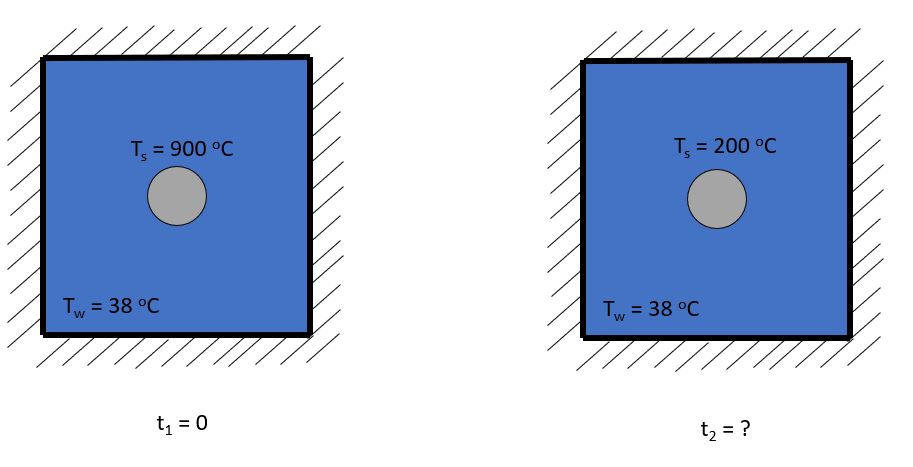
\includegraphics[width=0.85\textwidth]{part_a_fig}
	\caption{Part A schematic at initial and final state.}
	\label{fig:schem_a}
\end{figure}
\FloatBarrier
\subsection{Analysis}

Energy balance for closed system gives the following equation.
\begin{equation}\label{eqn_1}
	\stackrel{.}{Q} = hA(T_{s}-T_{f}) = C_{p}\rho V \frac{dT_{c}}{dt}
\end{equation}

Where $\stackrel{.}{Q}$ is energy flow [$W$], $h$ is the heat transfer coefficient [$W/m^{2}K$], $A$ is the surface area between the ball and water [$m^{2}$], $T_{s}$ is the temperature of the steel ball [$^{o}C$], $T_{f}$ is the temperature of the water [$^{o}C$], $C_{p}$ is the specific heat capacity [$J/mK$], $\rho$ is the density of the steel ball[$kg/m^{3}$], $V$ is the volume of the steel ball [$m^3$] and $t$ is the time [$s$].
\newline

Rearranging (\ref{eqn_1}) to separate the variables gives.
\begin{equation}\label{key}
	\frac{1}{T_{s}-T_{f}} dT_{c} = \frac{hA}{C_{p}\rho V}dt
\end{equation}

Which integrates to give.
\begin{equation}\label{eqn_3}
	\ln{(\frac{T_{s1}-T_{f}}{T_{s2}-T_{f}})} =  \frac{hA}{C_{p}\rho V}(t_{2}-t_{1})
\end{equation}
Where $t_{i}$ and $T_{si}$ are the time [s] and temperature [$^oC$] receptively at state i.

Rearranging (\ref{eqn_3}) to make $t_{2}$ the subject gives.
\begin{equation}\label{key}
	t_{2} = \frac{C_{p}\rho V}{hA}(\ln{(\frac{T_{s1}-T_{f}}{T_{s2}-T_{f}})})
\end{equation}

Substituting in the values for the variables given in Figure \ref{fig:schem_a} gives the final value.
\boldmath
\begin{equation}\label{key}
	t_2 = 205 s
\end{equation}
\unboldmath
Where $t_2$ is the time for the steel ball to reach a temperature of $200^{o}C$ under given assumptions.

\section{\emph{Part B: Lumped capacitance justification}}
\begin{equation}
	Bi = \frac{h L_{c}}{k}
\end{equation}
Where $h$ is conductivity [W/mK]
\begin{equation}
	t=\frac{f_{0} \rho C_{p} R^{2}}{k}
\end{equation}
\section{\emph{Part C: Transient conduction}}

\section{\emph{Part D: Non-infinite water bath}}

\section{\emph{Part E: Equilibrium temperature}}
\end{document}
